\lstinputlisting[language=bash,basicstyle=\small]{python_codes/fieldstone_14/keywords}

\begin{center}
Code at \url{https://github.com/cedrict/fieldstone/tree/master/python_codes/fieldstone_14}
\end{center}

\par\noindent\rule{\textwidth}{0.4pt}
%%%%%%%%%%%%%%%%%%%%%%%%%%%%%%%%%%%%%%%%%%%%%%%%%%%%%%%%%%%%%%%%%%%%%%%%%%%%%%%%%%%%%%%%%%%%

The details of the numerical setup are presented in Section~\ref{mms1}.

In this stone we do not use the penalty formulation and therefore 
keep both velocity and pressure as unknowns. Therefore we end up having to solve 
the following saddle point system:
\[
\left(
\begin{array}{cc}
\K & \G \\ \G^T & 0 
\end{array}
\right)
\cdot
\left(
\begin{array}{c}
V \\ P
\end{array}
\right)
=
\left(
\begin{array}{c}
 f \\ h
\end{array}
\right)
\quad\quad
{\rm or,}
\quad\quad
\A \cdot X = rhs
\]
Each block $\K$, $\G$ and vector $f$, $h$ is built separately for each element 
in the code and assembled into 
the matrix $\A$ and vector $rhs$ afterwards. $\A$ and $rhs$ are then passed to the solver. 

Each element has $m_\upnu=4$ vertices so in total $ndofV\times m_\upnu=8$ 
velocity dofs and a single 
pressure dof, commonly situated in the center of the element. The total number of 
velocity dofs is therefore $NfemV=NV \times ndofV$ while the total number of
pressure dofs is $NfemP=nel$. The total number of dofs is then $Nfem=NfemV+NfemP$.

As a consequence, matrix $\K$ has size $(NfemV,NfemV)$ and matrix $\G$ has size $(NfemV,NfemP)$.
Vector $f$ is of size $NfemV$ and vector $h$ is of size $NfemP$.  

The pressure nullspace is removed by imposing that $\int_\Omega p \; dV =0$ through 
a Lagrange multiplier (see Section~\ref{ss_pnorm}).

\begin{center}
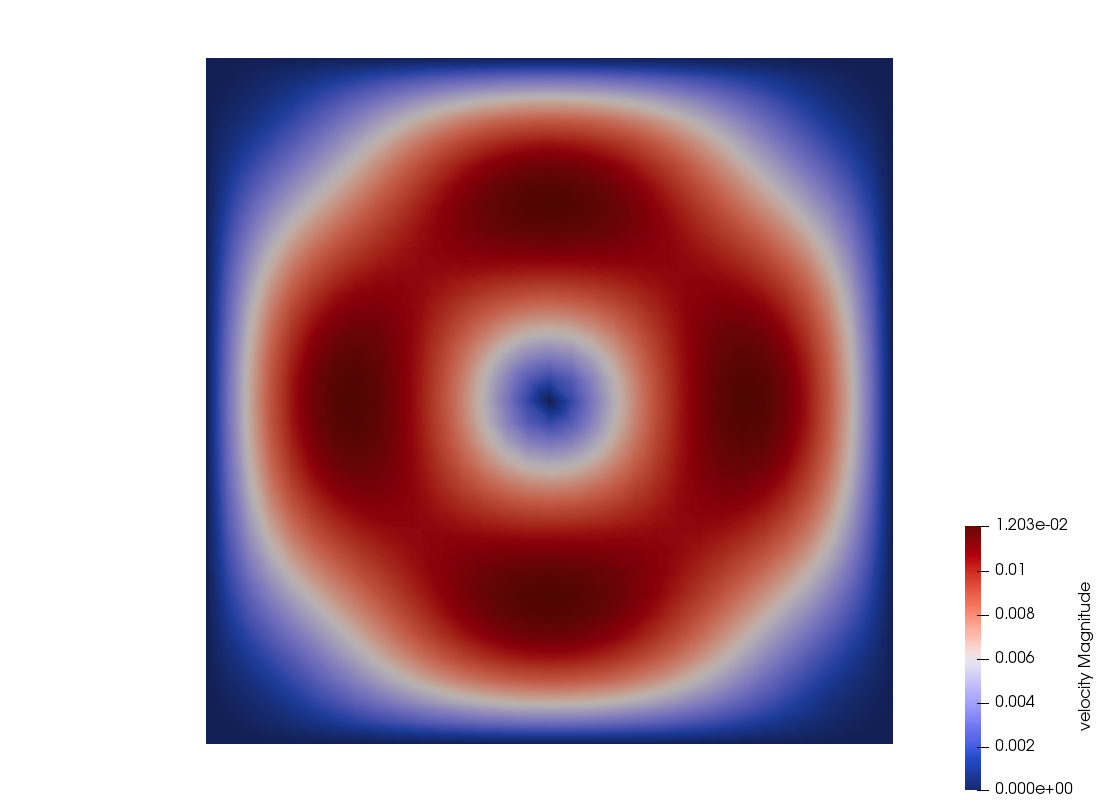
\includegraphics[width=5.6cm]{python_codes/fieldstone_14/results/vel}
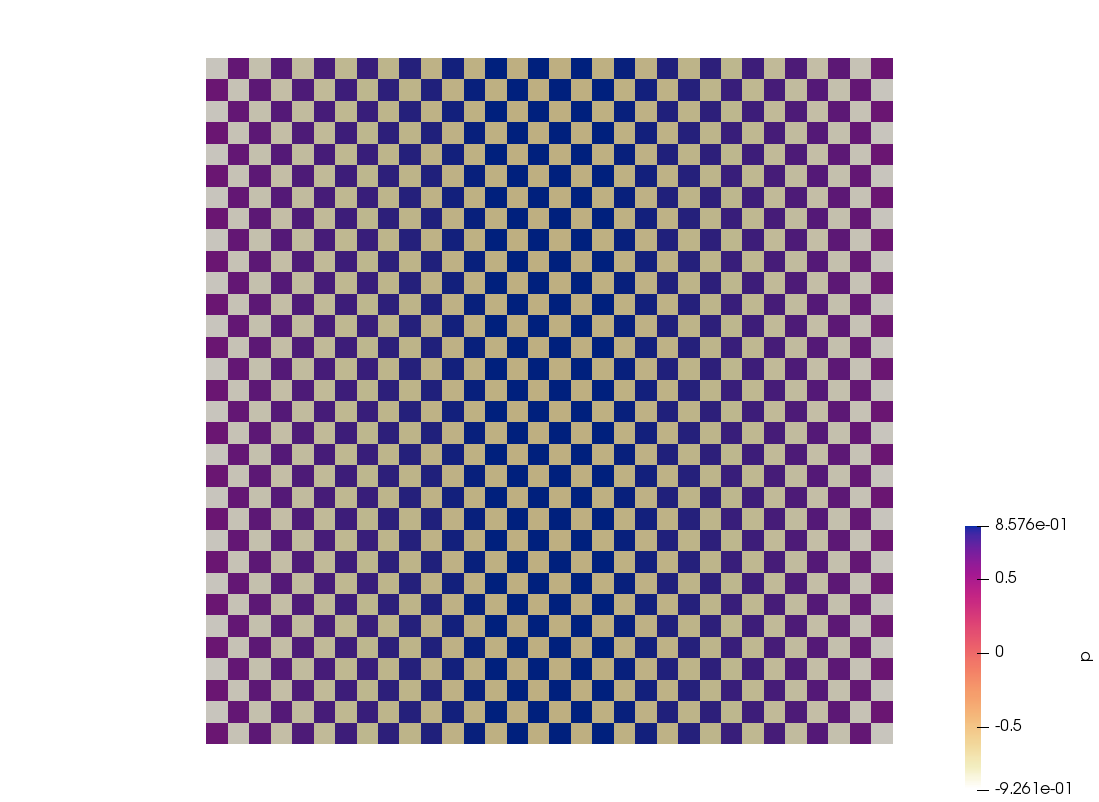
\includegraphics[width=5.6cm]{python_codes/fieldstone_14/results/p}
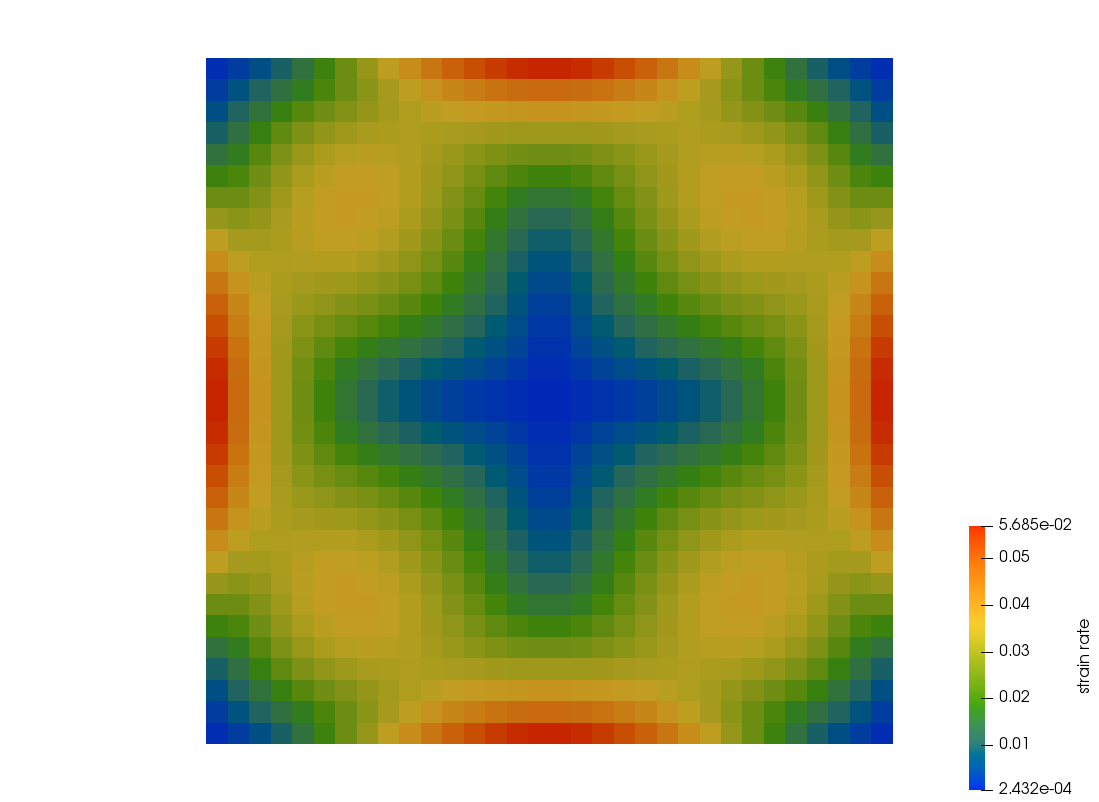
\includegraphics[width=5.6cm]{python_codes/fieldstone_14/results/sr}\\
{\captionfont From left to right: velocity, pressure and second invariant 
of strain rate for 32x32 mesh.}
\end{center}

Unlike the results obtained with the penalty formulation (see Section \ref{f1}),
the pressure showcases a very strong checkerboard pattern, similar to the one 
in \cite{dohu03}. The amplitude of this checkerboard is unpredictable 
and changes from one resolution to the other.

\begin{center}
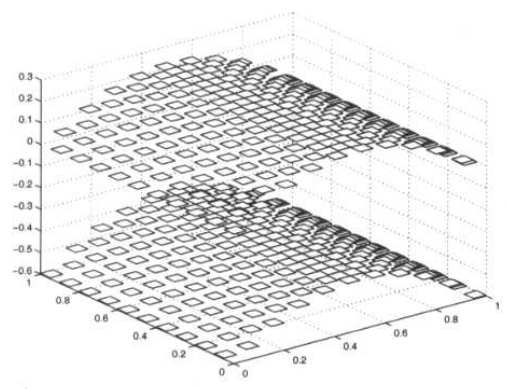
\includegraphics[width=5.6cm]{python_codes/fieldstone_14/results/doneahuerta}
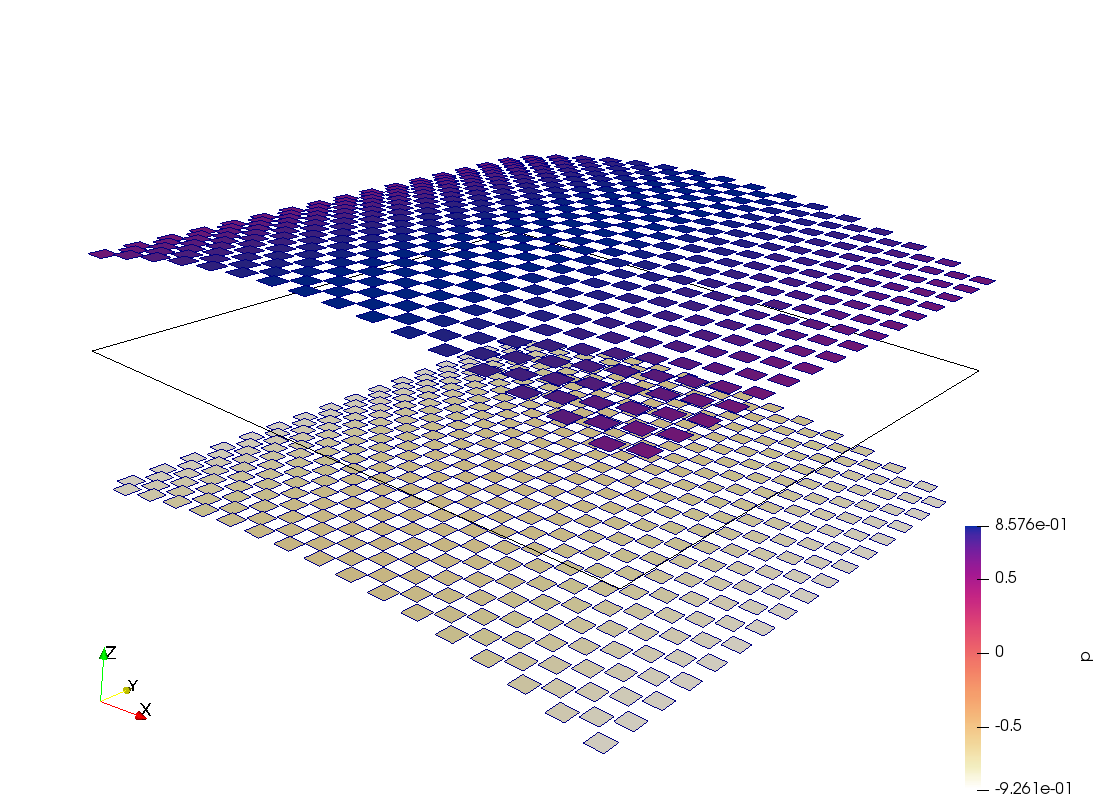
\includegraphics[width=5.6cm]{python_codes/fieldstone_14/results/p_3D}
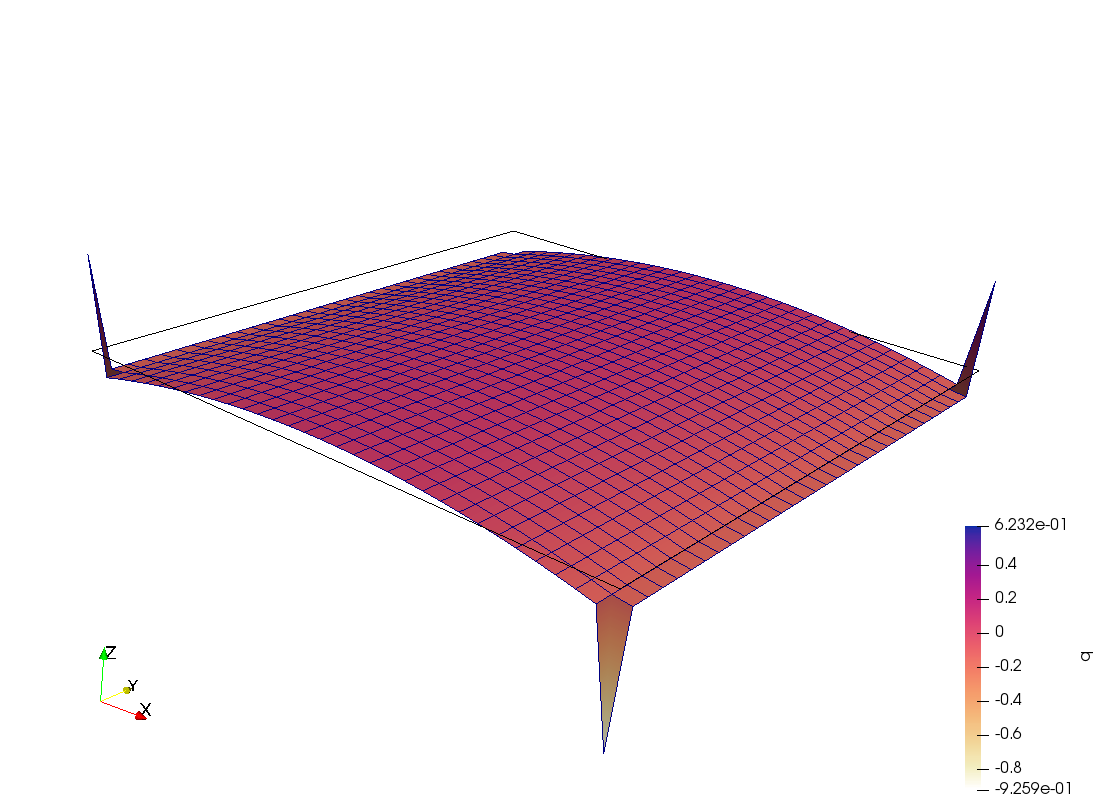
\includegraphics[width=5.6cm]{python_codes/fieldstone_14/results/q_3D}\\
{\captionfont Left: pressure solution as shown in \cite{dohu03}; Right: elemental 
pressure solution obtained with fieldstone on a 32x32 grid. 
Note that the vtu file was build in such a way so as to allow for 
this representation of the discontinuous pressure field.}
\end{center}

The nodal pressure (obtained with a simple center-to-node algorithm)
fails to recover a correct pressure at the four corners.

I have also explored the two formulations for the ${\bm C}$ matrix needed to 
compute $\K$ (see Section~\ref{sec:mixed}):
\[
{\bm C}^{(a)}= \eta 
\left(
\begin{array}{ccc}
2 & 0 & 0 \\
0 & 2 & 0 \\
0 & 0 & 1
\end{array}
\right)
\qquad
{\bm C}^{(b)}= \eta
\left(
\begin{array}{ccc}
4/3 & -2/3 & 0 \\
-2/3 & 4/3 & 0 \\
0 & 0 & 1
\end{array}
\right)
\]
It seems that option $b$ yields slightly better velocity accuracy, but the pressure 
checkerboard derails pressure error measurements for both cases:

\begin{center}
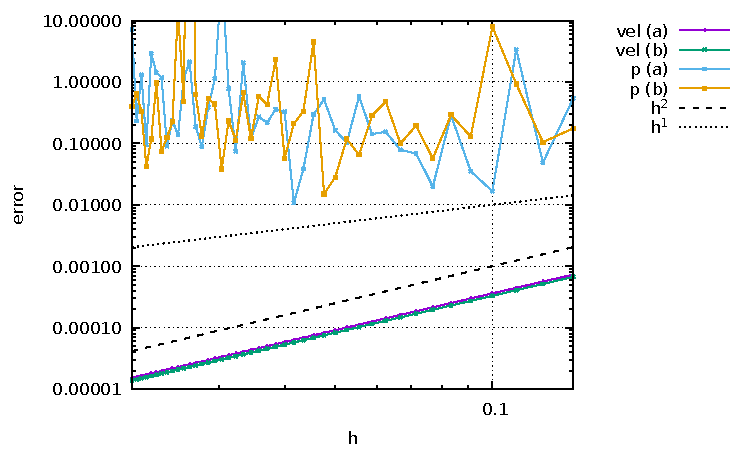
\includegraphics[width=11cm]{python_codes/fieldstone_14/results/errors.pdf}
\end{center}


\begin{center}
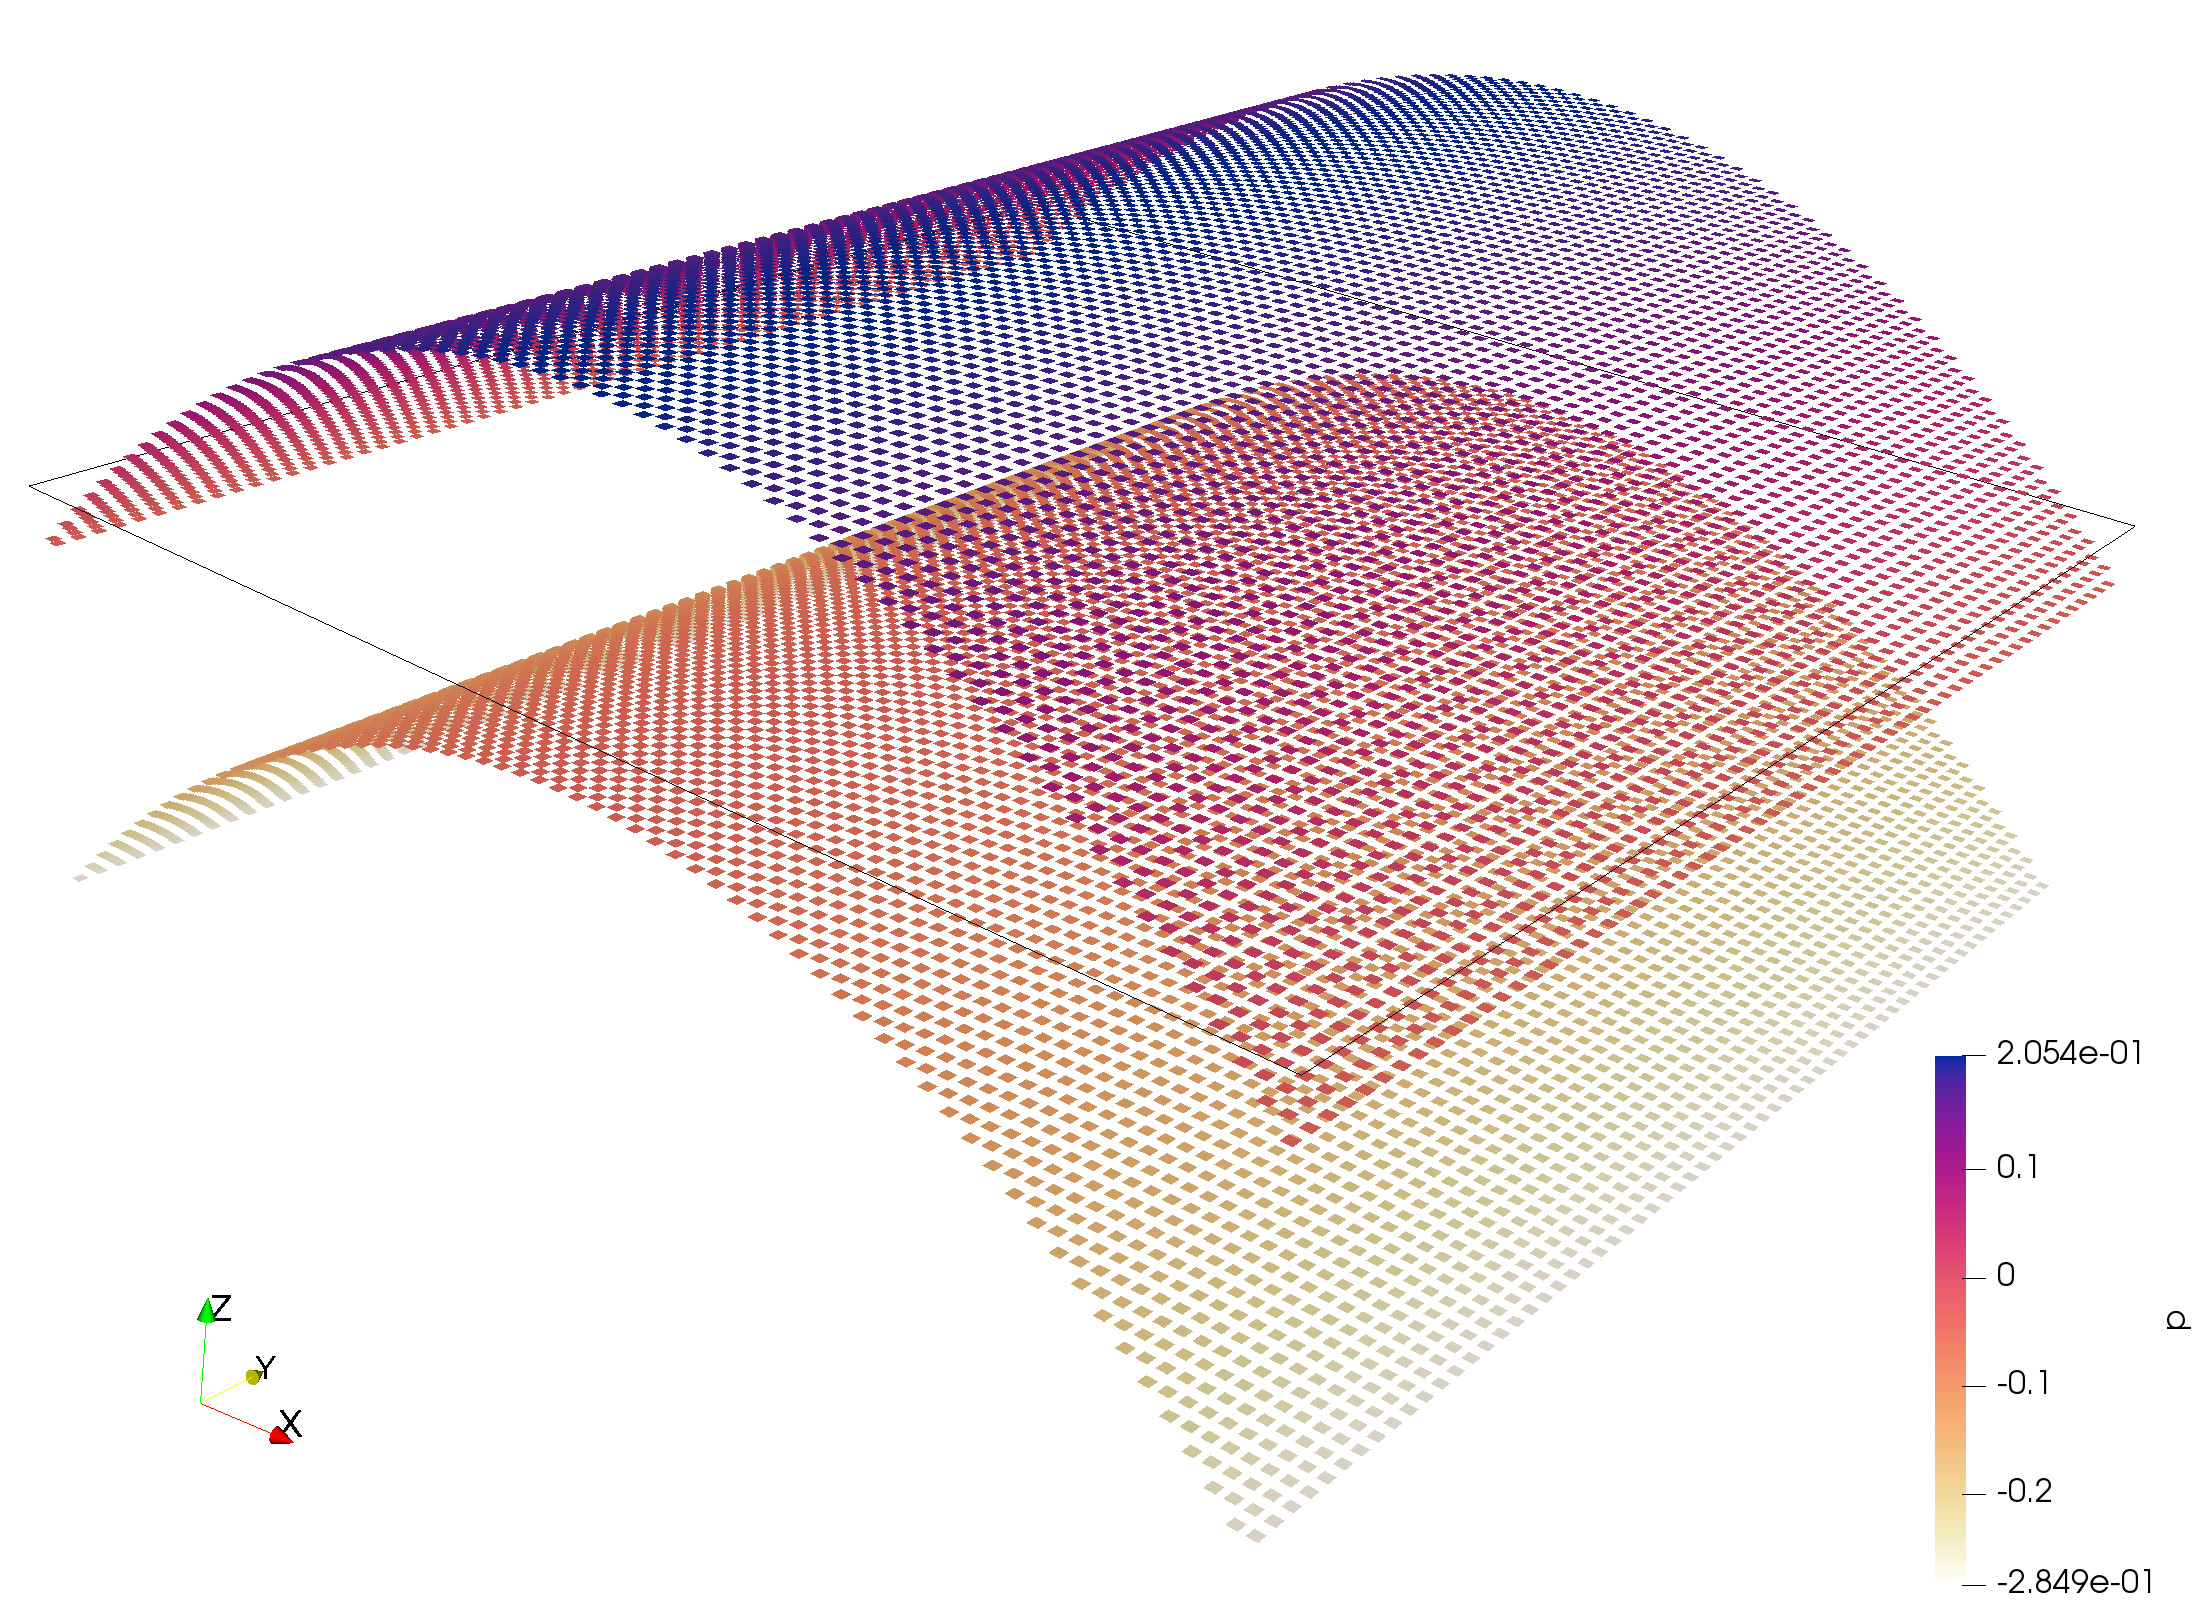
\includegraphics[width=15cm]{python_codes/fieldstone_14/results/p128x128}\\
{\captionfont Elemental pressure for 128x128 mesh.}
\end{center}
